\chapter{Arhitektura i dizajn sustava}
		
		\textbf{\textit{dio 1. revizije}}\\

		\textit{ Potrebno je opisati stil arhitekture te identificirati: podsustave, preslikavanje na radnu platformu, spremišta podataka, mrežne protokole, globalni upravljački tok i sklopovsko-programske zahtjeve. Po točkama razraditi i popratiti odgovarajućim skicama:}
	\begin{itemize}
		\item 	\textit{izbor arhitekture temeljem principa oblikovanja pokazanih na predavanjima (objasniti zašto ste baš odabrali takvu arhitekturu)}
		\item 	\textit{organizaciju sustava s najviše razine apstrakcije (npr. klijent-poslužitelj, baza podataka, datotečni sustav, grafičko sučelje)}
		\item 	\textit{organizaciju aplikacije (npr. slojevi frontend i backend, MVC arhitektura) }		
	\end{itemize}

	
		

		

				
		\section{Baza podataka}
			
			\textbf{\textit{dio 1. revizije}}\\
			
		\textit{Potrebno je opisati koju vrstu i implementaciju baze podataka ste odabrali, glavne komponente od kojih se sastoji i slično.}
		
			\subsection{Opis tablica}
			

				\textit{Svaku tablicu je potrebno opisati po zadanom predlošku. Lijevo se nalazi točno ime varijable u bazi podataka, u sredini se nalazi tip podataka, a desno se nalazi opis varijable. Svjetlozelenom bojom označite primarni ključ. Svjetlo plavom označite strani ključ}
				
				
				\begin{longtblr}[
					label=none,
					entry=none
					]{
						width = \textwidth,
						colspec={|X[6,l]|X[6, l]|X[20, l]|}, 
						rowhead = 1,
					} %definicija širine tablice, širine stupaca, poravnanje i broja redaka naslova tablice
					\hline \SetCell[c=3]{c}{\textbf{korisnik - ime tablice}}	 \\ \hline[3pt]
					\SetCell{LightGreen}IDKorisnik & INT	&  	Lorem ipsum dolor sit amet, consectetur adipiscing elit, sed do eiusmod  	\\ \hline
					korisnickoIme	& VARCHAR &   	\\ \hline 
					email & VARCHAR &   \\ \hline 
					ime & VARCHAR	&  		\\ \hline 
					\SetCell{LightBlue} primjer	& VARCHAR &   	\\ \hline 
				\end{longtblr}
				
				
			
			\subsection{Dijagram baze podataka}
				\textit{ U ovom potpoglavlju potrebno je umetnuti dijagram baze podataka. Primarni i strani ključevi moraju biti označeni, a tablice povezane. Bazu podataka je potrebno normalizirati. Podsjetite se kolegija "Baze podataka".}
			
			\eject
			
			
		\section{Dijagram razreda}
		
			{Na sljedećim slikama prikazani su dijagrami razreda koji se odnose na \textit{backend} dio aplikacije. Na slici 4.1 prikazan je cjelokupni dijagram razreda, a na ostalima su razdvojeni u smislene cjeline. U implementaciji korištena je \textit{Spring Boot} tehnologija. Postoje tri sloja aplikacije: \textit{Controller}(REST API), \textit{Service}(poslovna logika) te \textit{Repository}(pristup podacima). }\\
			
			\begin{figure}[H]
				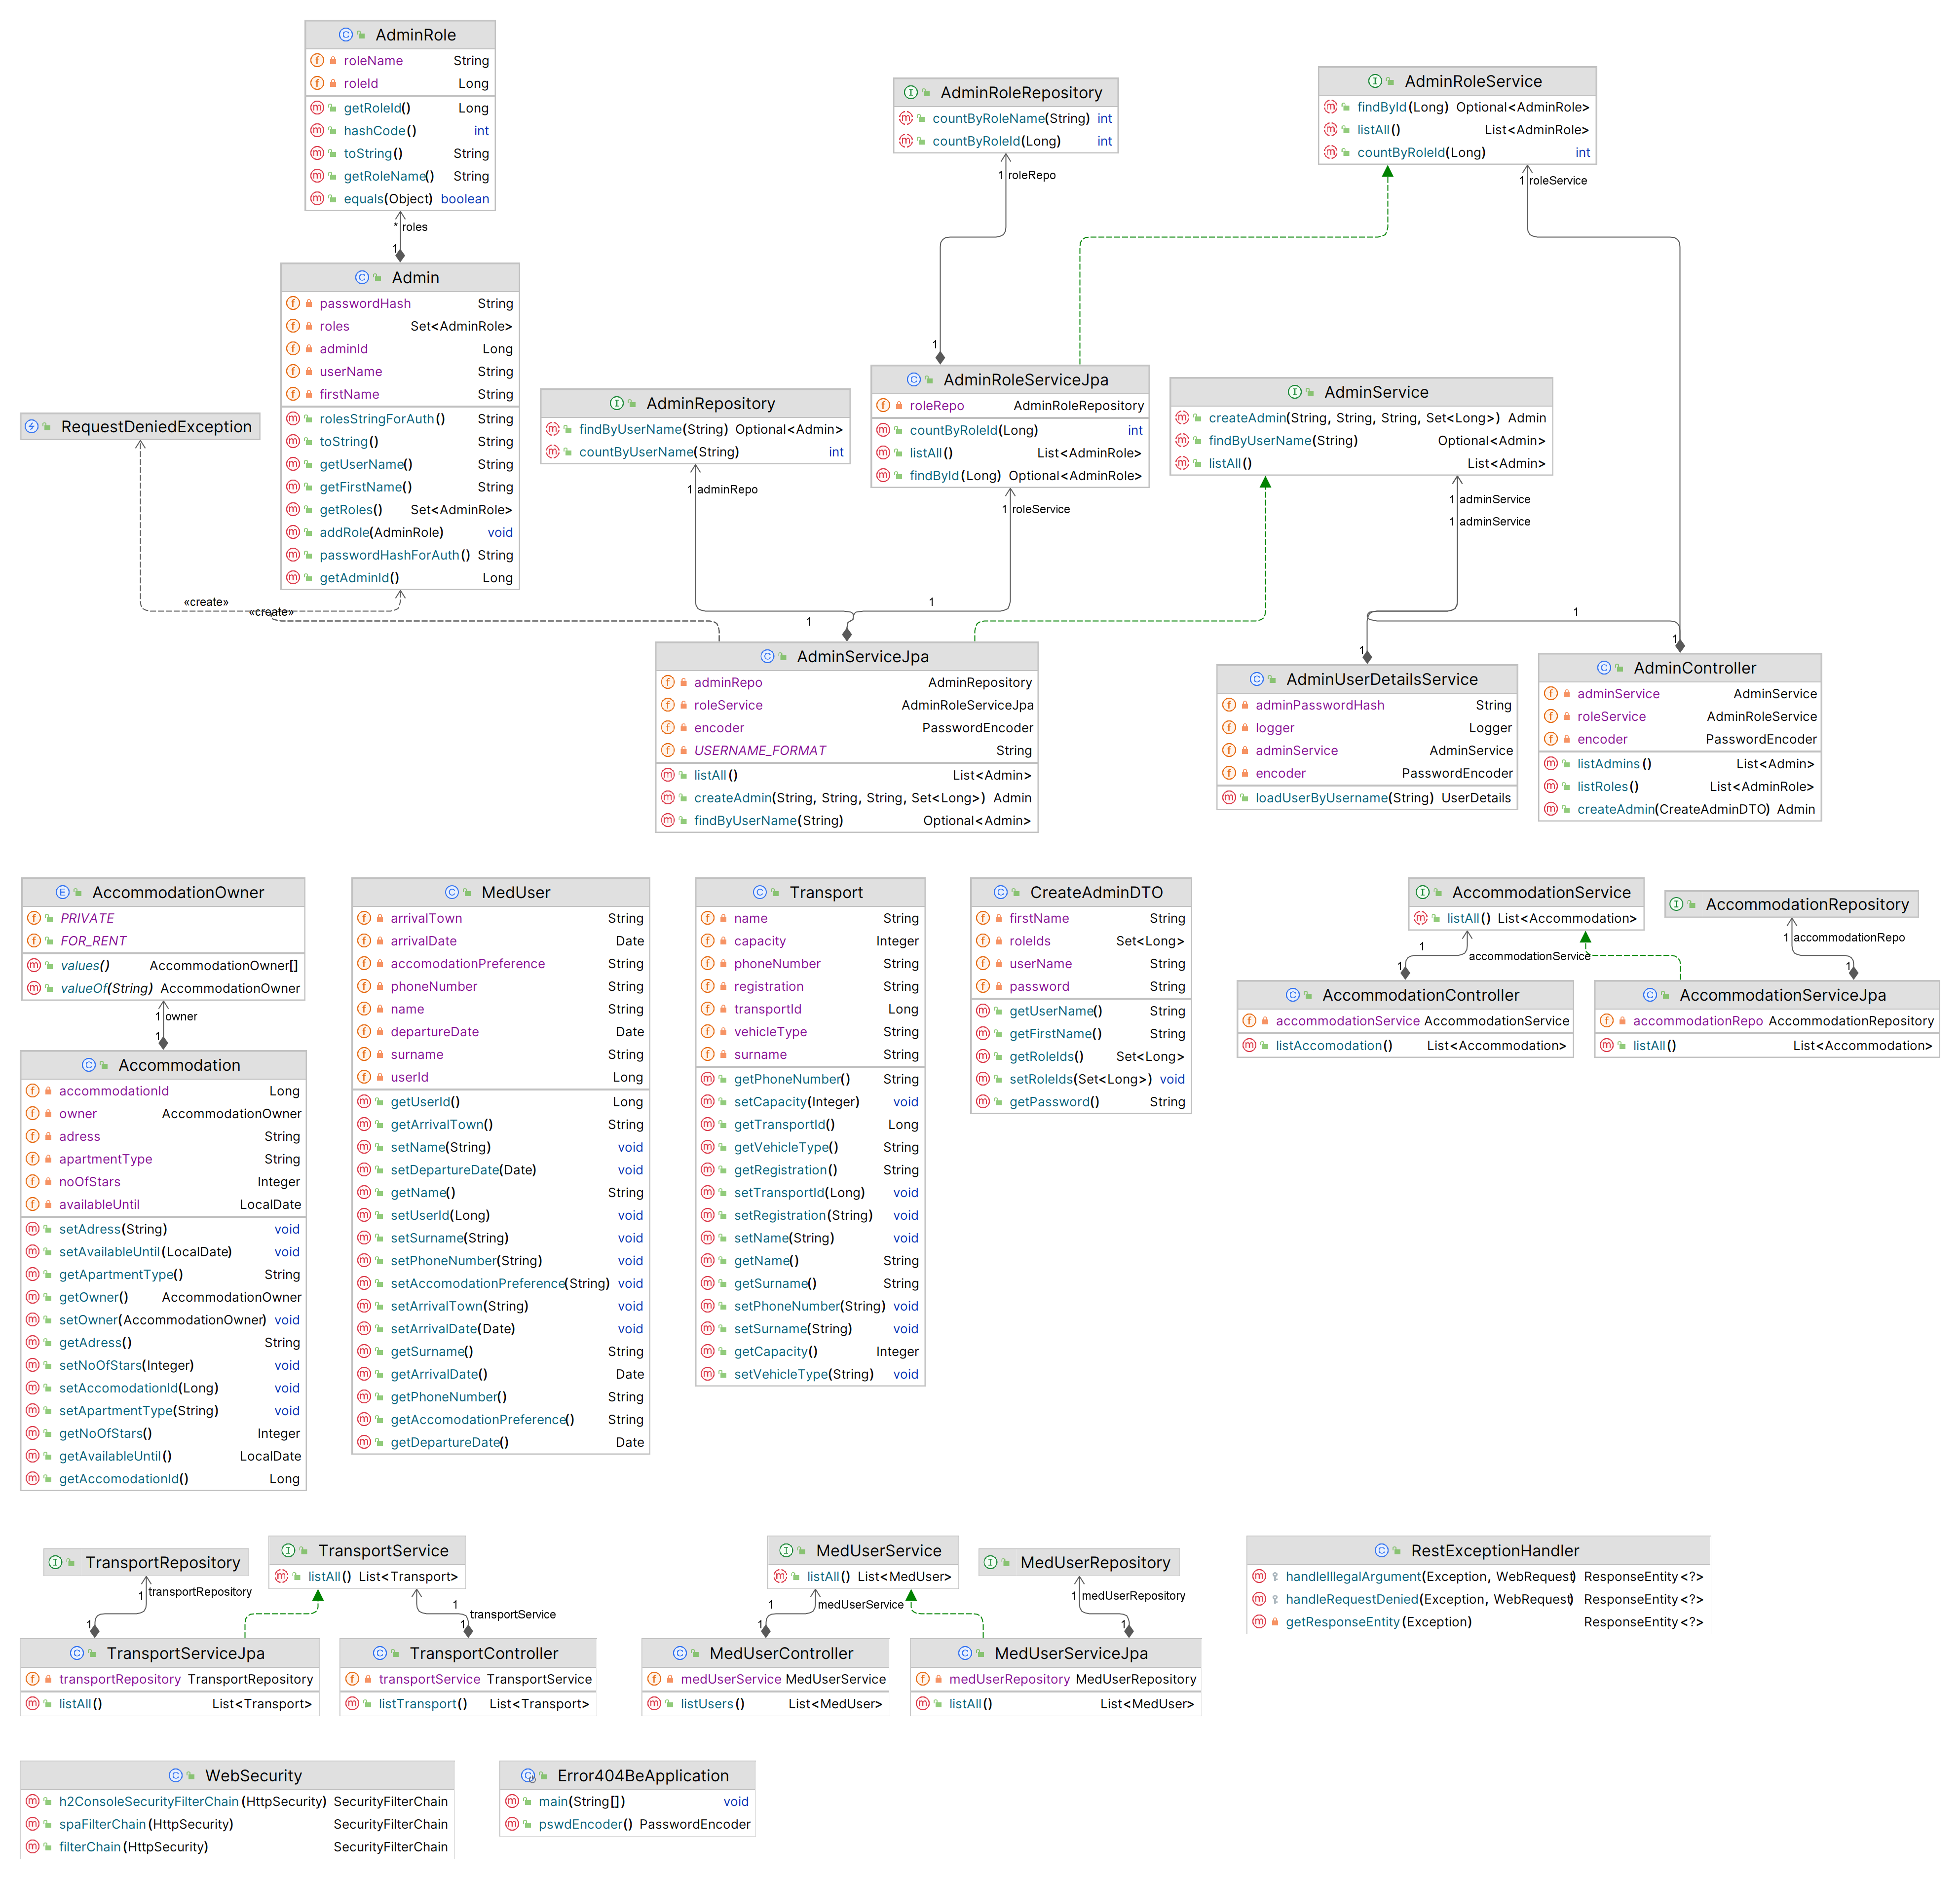
\includegraphics[width=\textwidth]{slike/CjelokupanDijagramRazreda.PNG}
				\caption{Cjelokupan dijagram razreda}
				\label{classDiagram}
			\end{figure}
			
			\begin{figure}[H]
				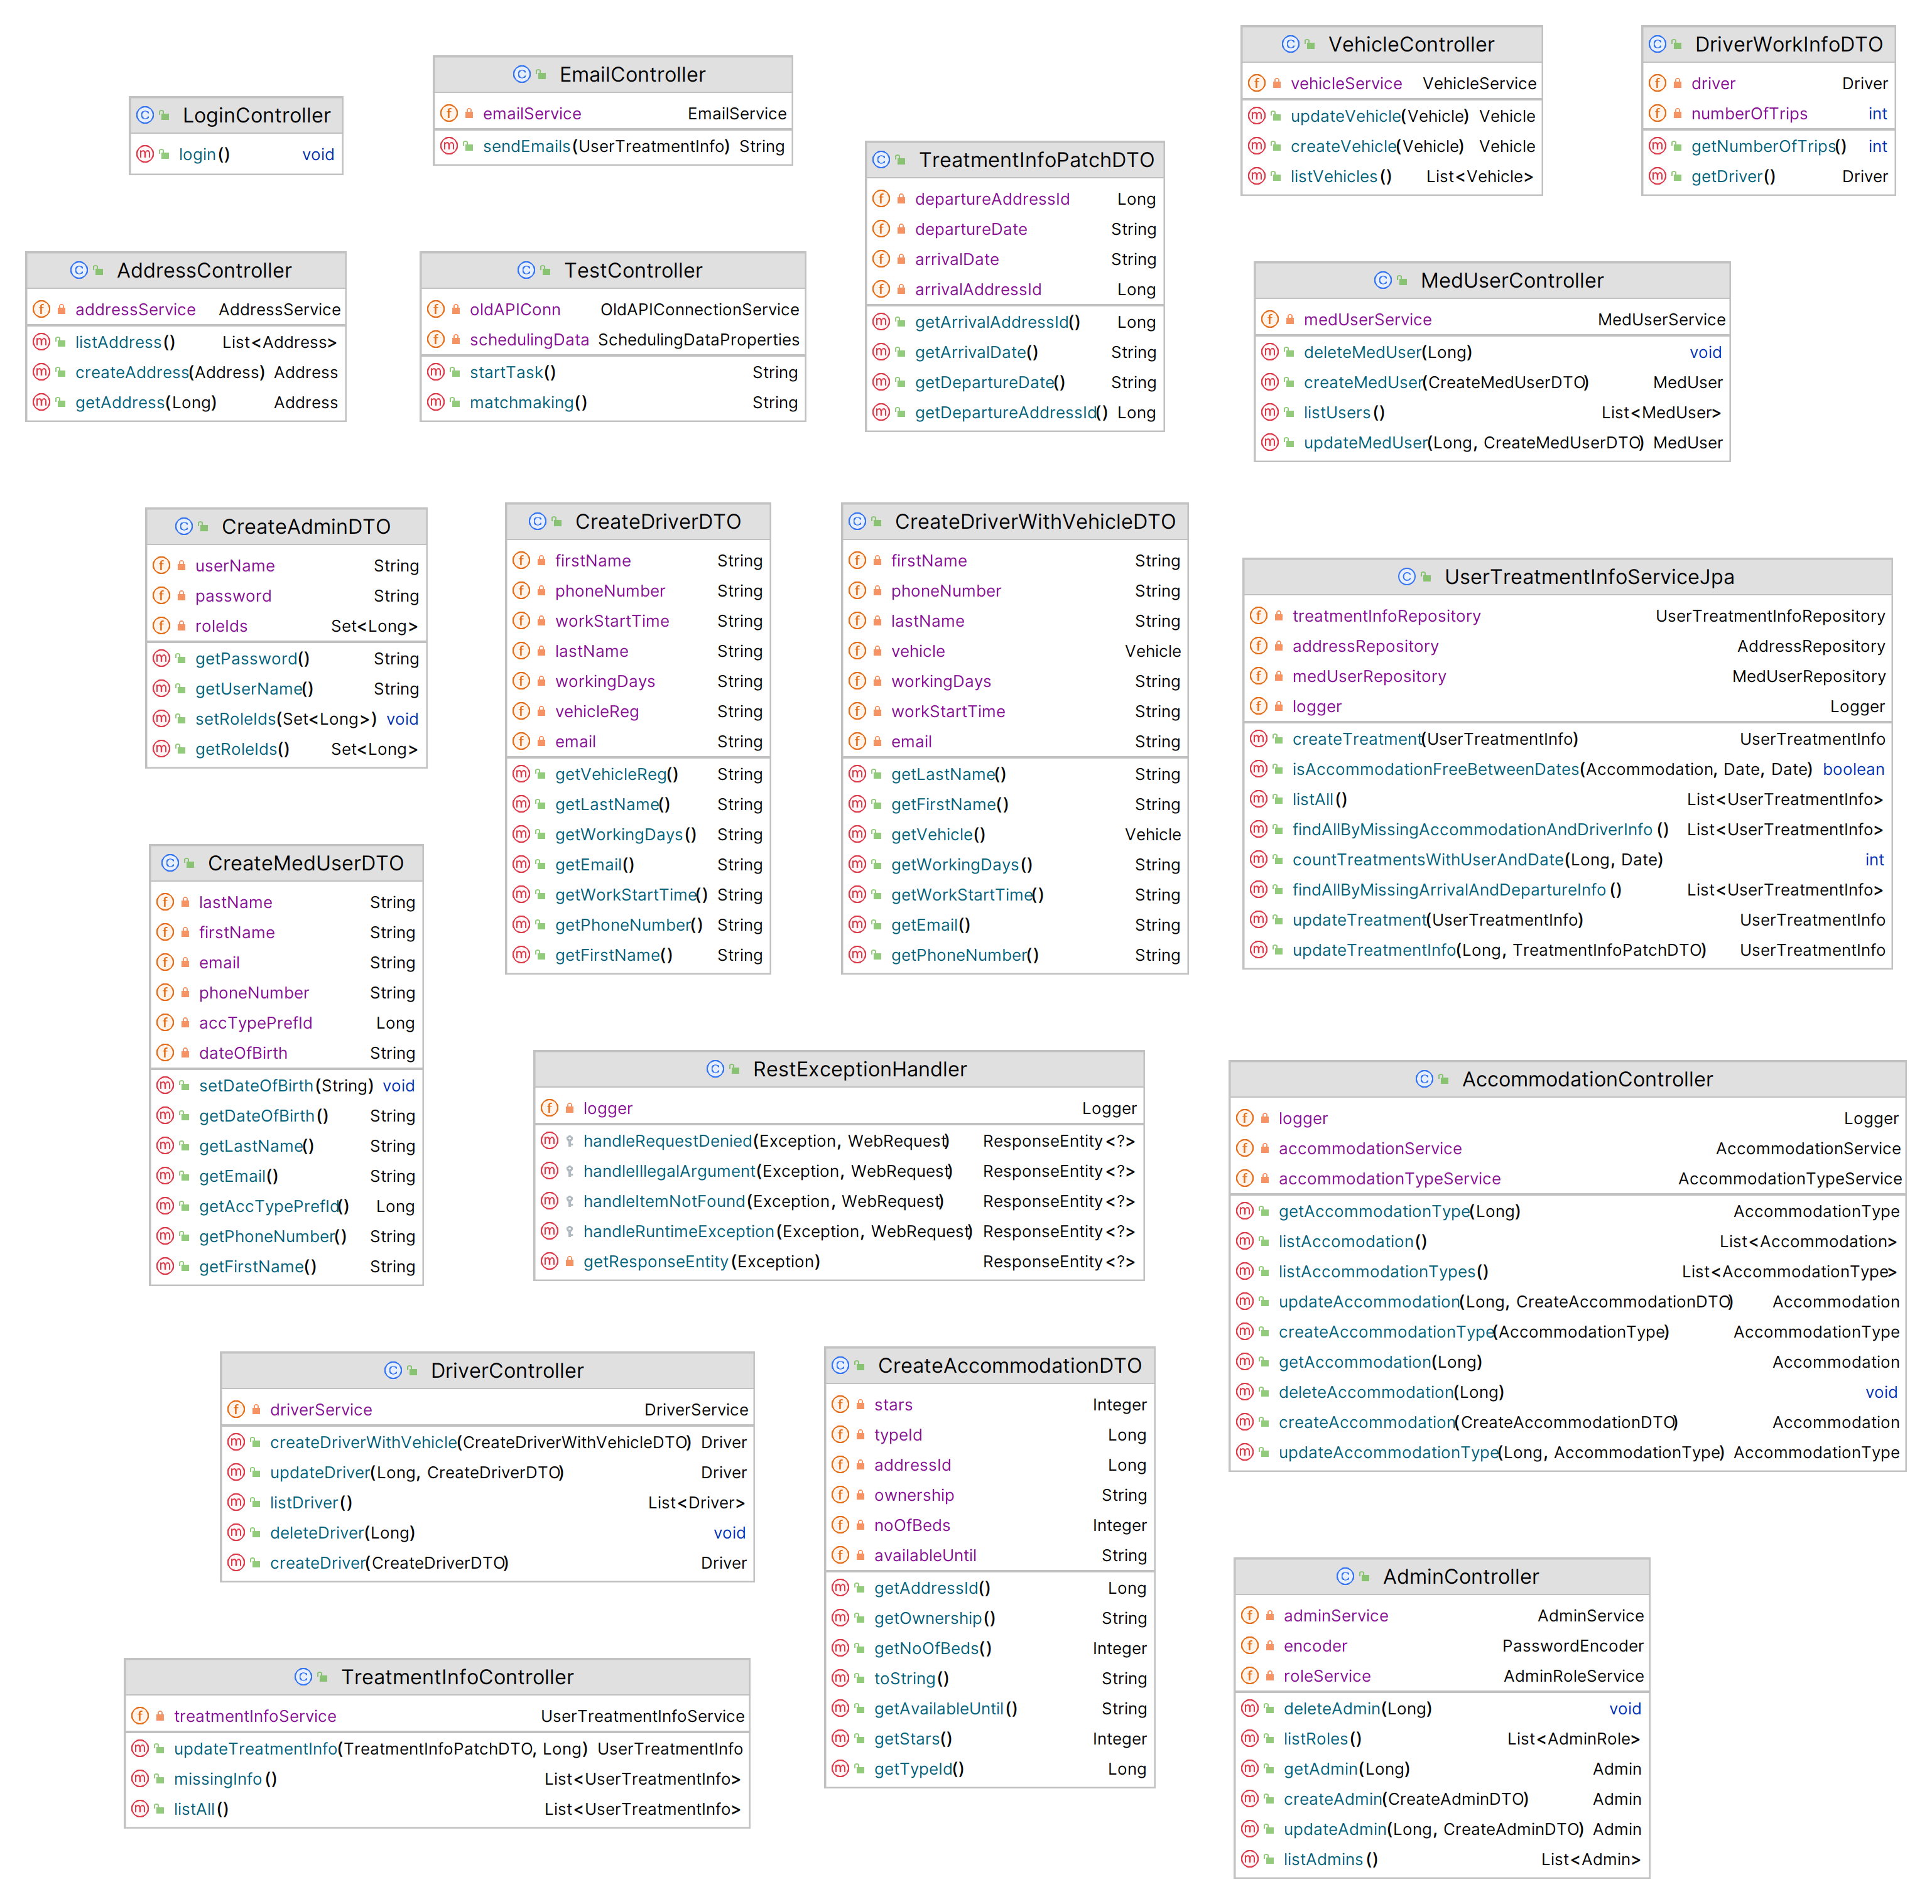
\includegraphics[width=\textwidth]{slike/rest.PNG}
				\caption{Dijagram razreda - Controller}
				\label{restDiagram}
			\end{figure}
			
			{Navedene klase nasljeđuju REST Controller koji je zadužen za rukovanje HTTP zahtjevima i za pružanje odgovarajućih odgovora. REST Controller vraća podatke u JSON formatu. \\ 
			CreateAdminDTO je \textit{Data transfer Object} koji je zadužen za stvaranje administratora. \textit{DTO} služi za transfer podataka između slojeva aplikacije, pogotovo između klijenta i servera. \\
			AdminUserDetailsService je \textit{Spring service} komponenta koja služi za baratanje detaljima administratora tijekom prijave i prilagođavanje korisničkih detalja na temelju odgovarajućih uloga i vjerodajnica, te osiguravanje sigurnosti}\\
			
			\begin{figure}[H]
				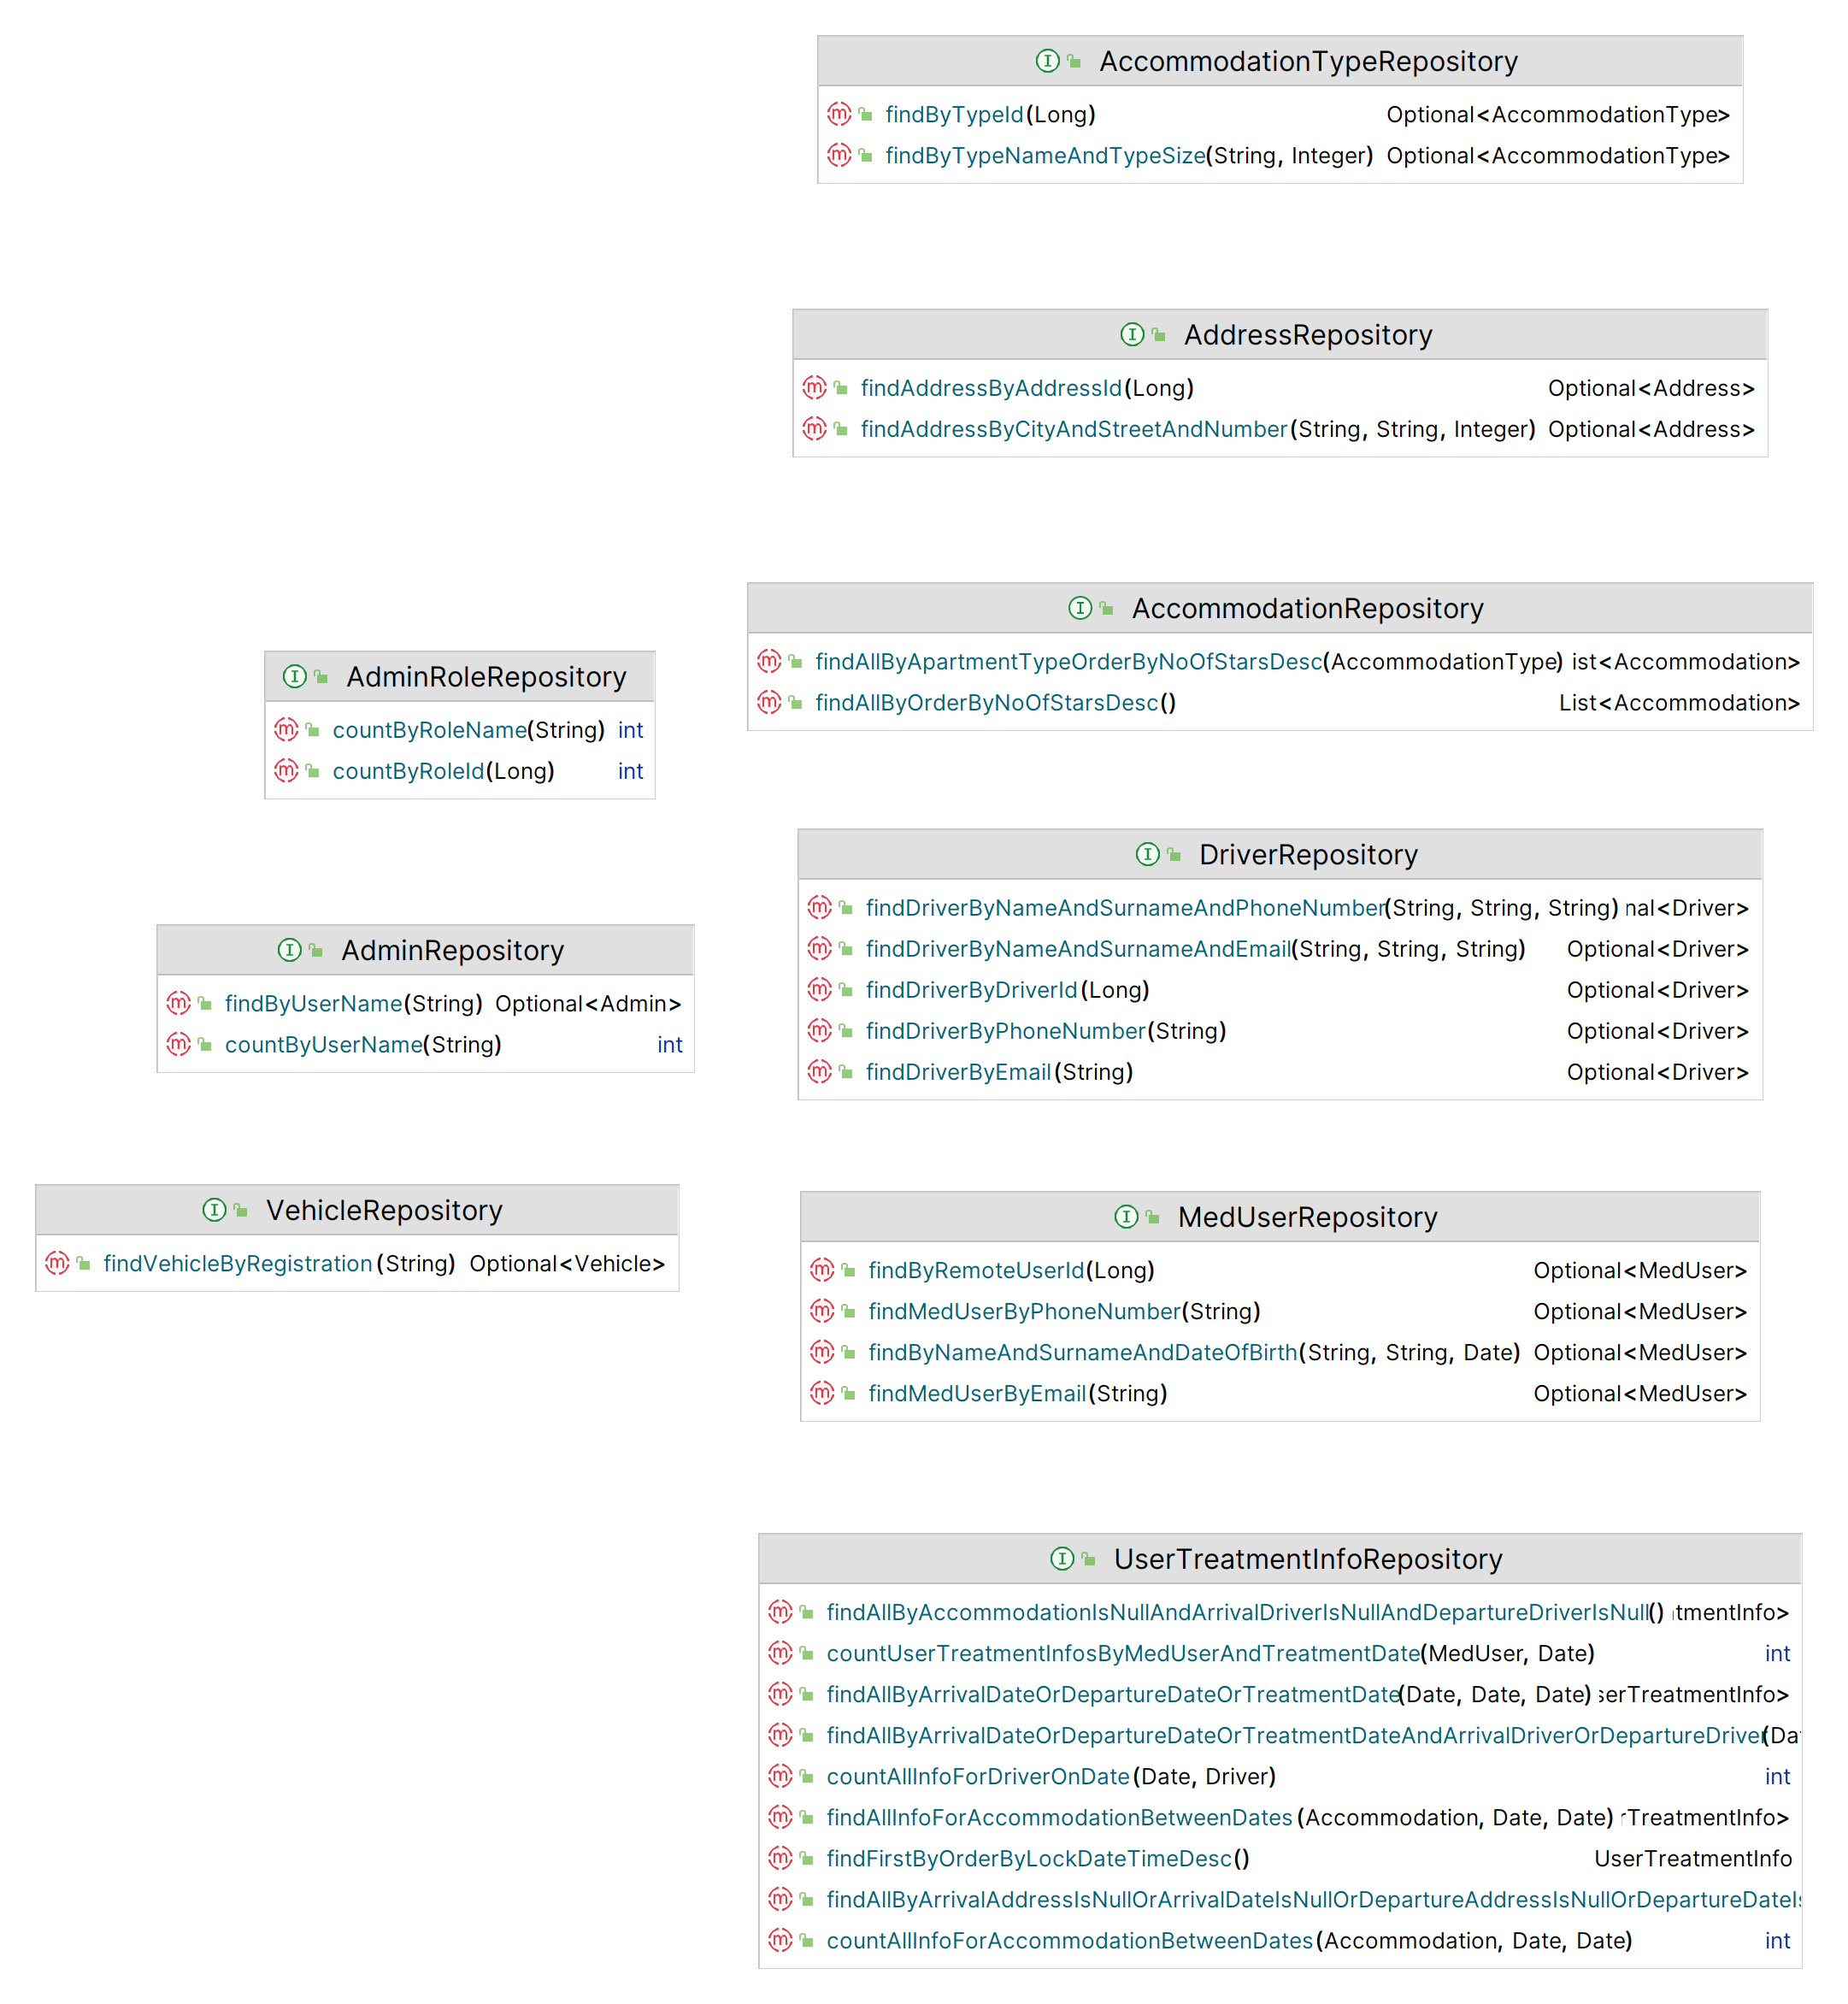
\includegraphics[width=\textwidth]{slike/dao.PNG}
				\caption{Dijagram razreda - Repository}
				\label{repositoryDiagram}
			\end{figure}
			
			{Navedena sučelja nasljeđuju \textit{JPARepository} koji pruža generičke metode za operacije s podatcima, poput spremanja, ažuriranja, brisanja i slično.}\\
			
			\begin{figure}[H]
				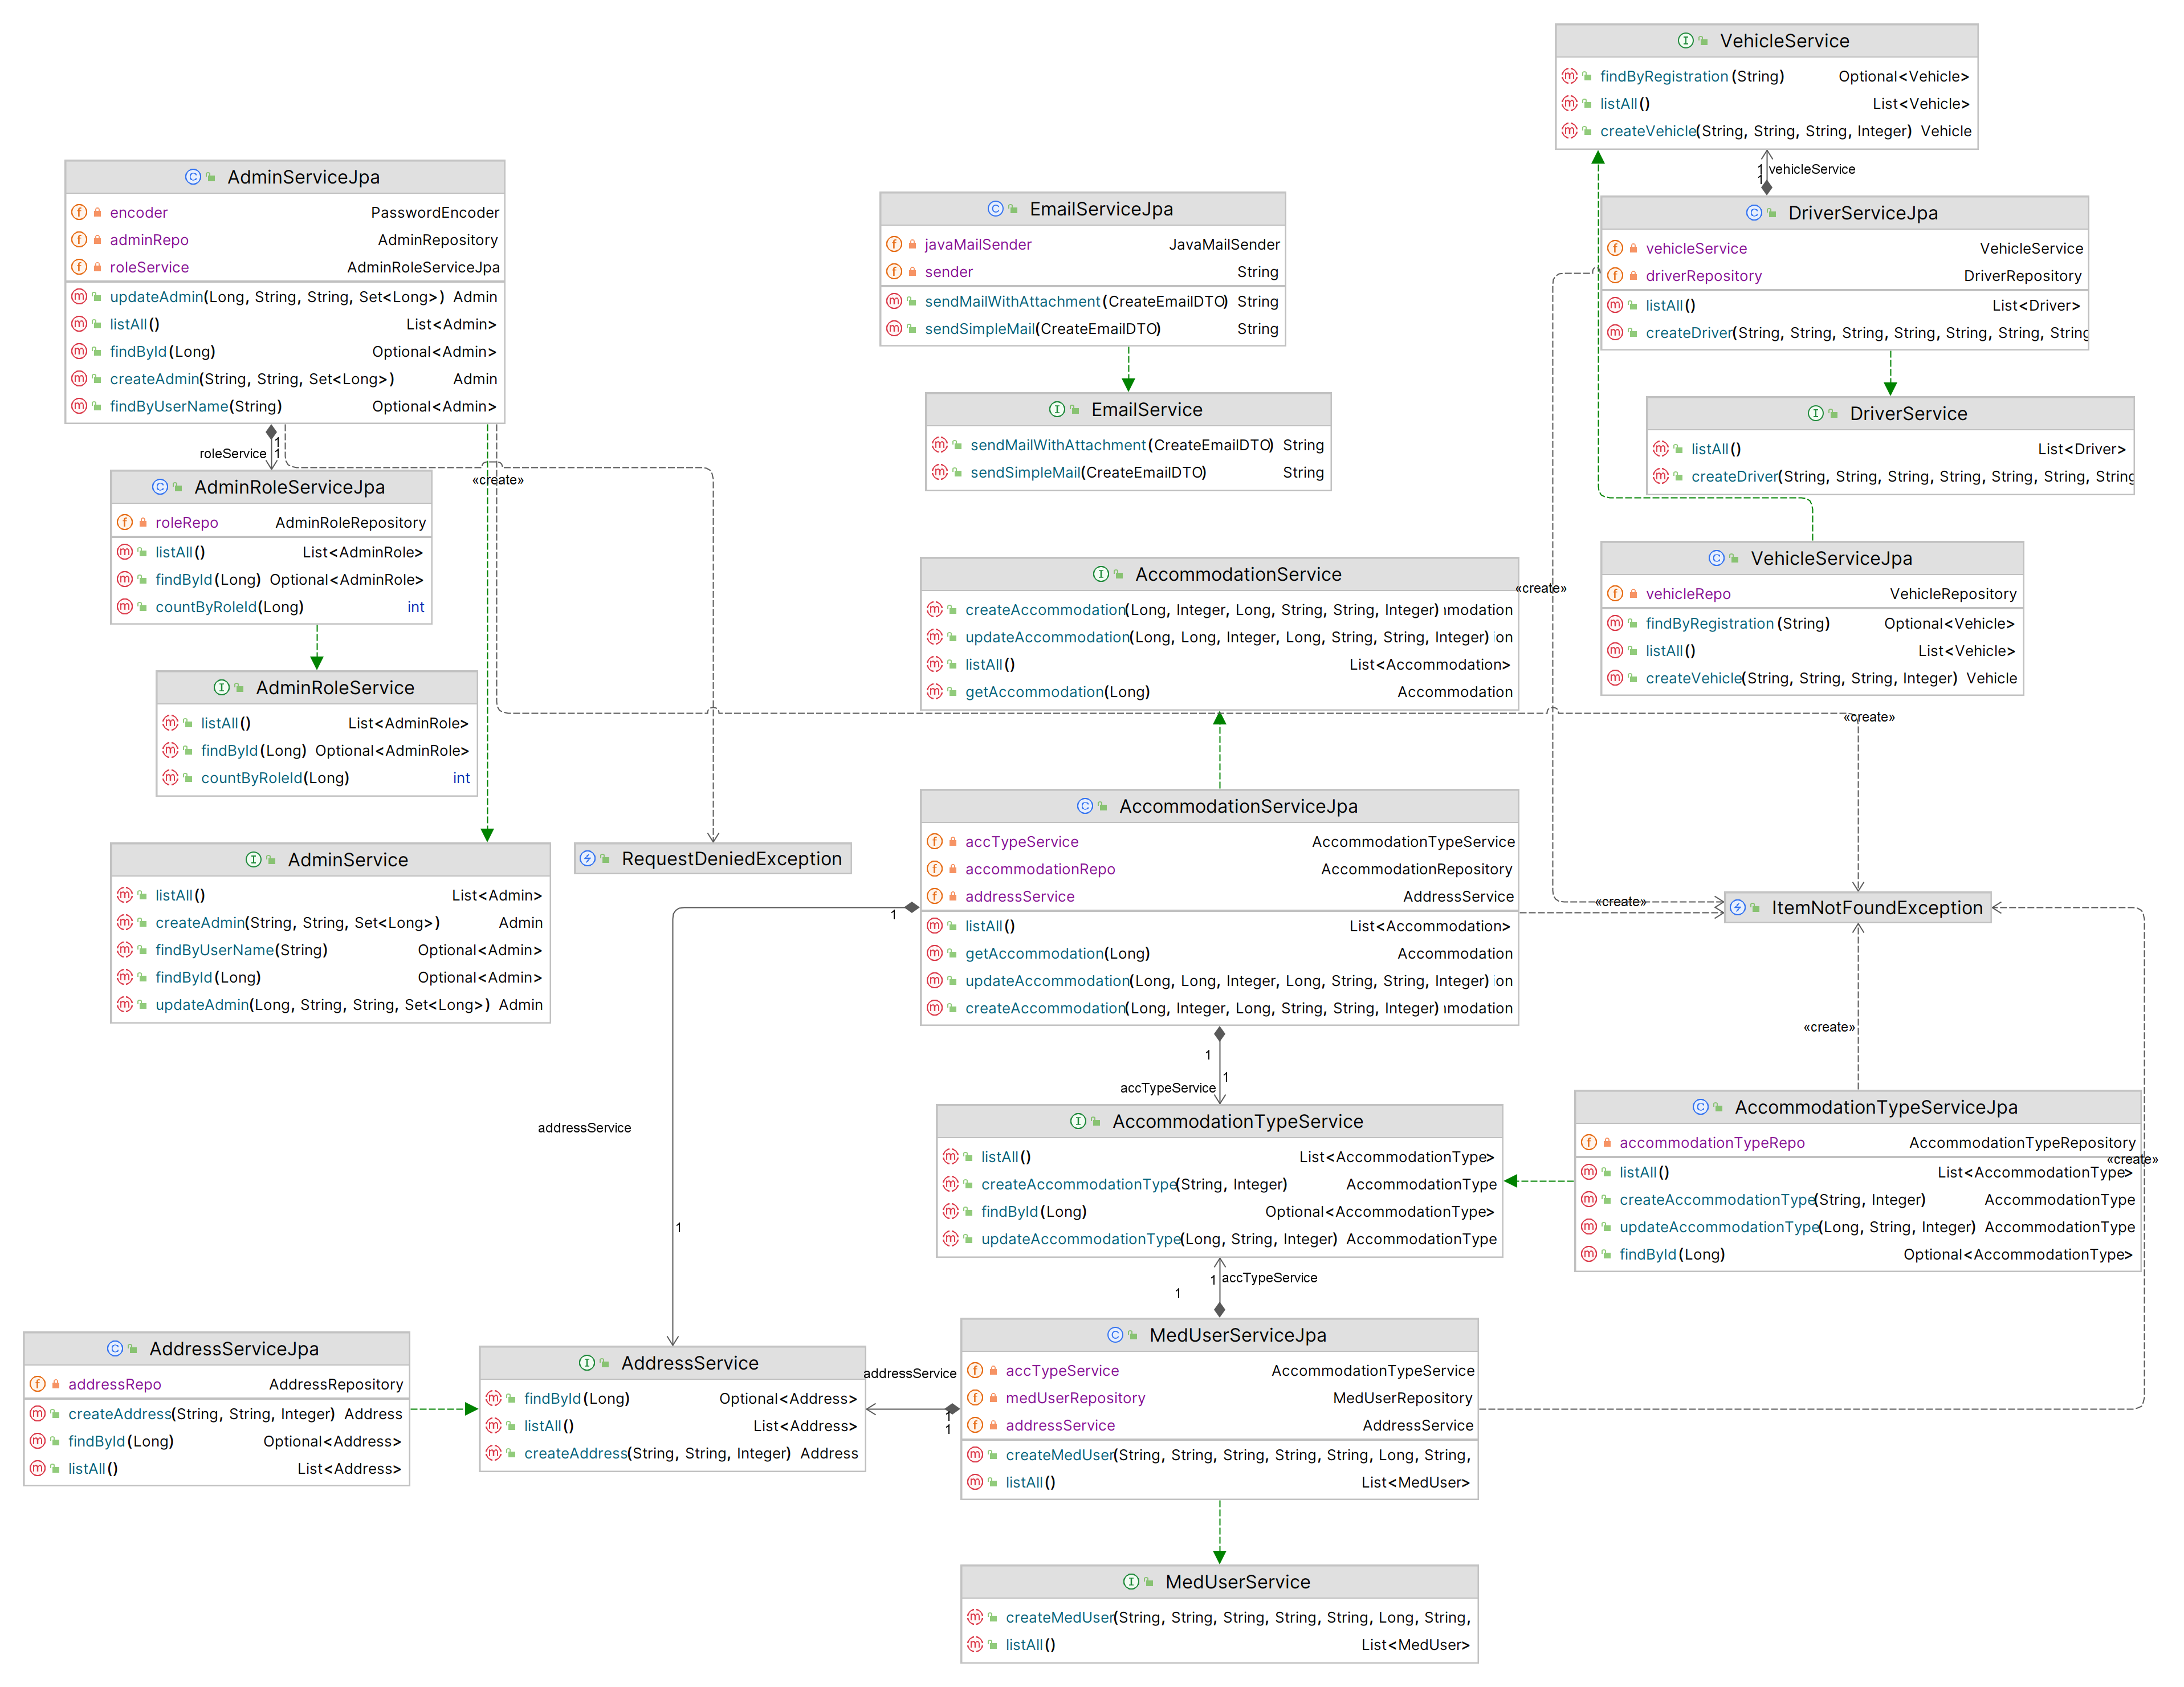
\includegraphics[width=\textwidth]{slike/service.PNG}
				\caption{Dijagram razreda - Service}
				\label{serviceDiagram}
			\end{figure}
			
			{Navedene \textit{Service} klase su \textit{Spring Service} klase, sadrže poslovnu logiku aplikacije, tj. odgovorni su za obradu podataka, implementaciju algoritama itd. Ponašaju se kao sloj između \textit{Controllera} i \textit{Repositoryja}.\\
			\textit{AdminService} sadrži metodu \textit{createAdmin} za stvaranje administratora. Postoji provjera raznih svojstava, poput duljine lozinke, duljine nadimka, postoji li već neki administrator s tim nadimkom, postojanje navedenih uloga itd. Ako je sve uspješno sprema se novi administrator u \textit{AdminRepository}.}\\
			
			\begin{figure}[H]
				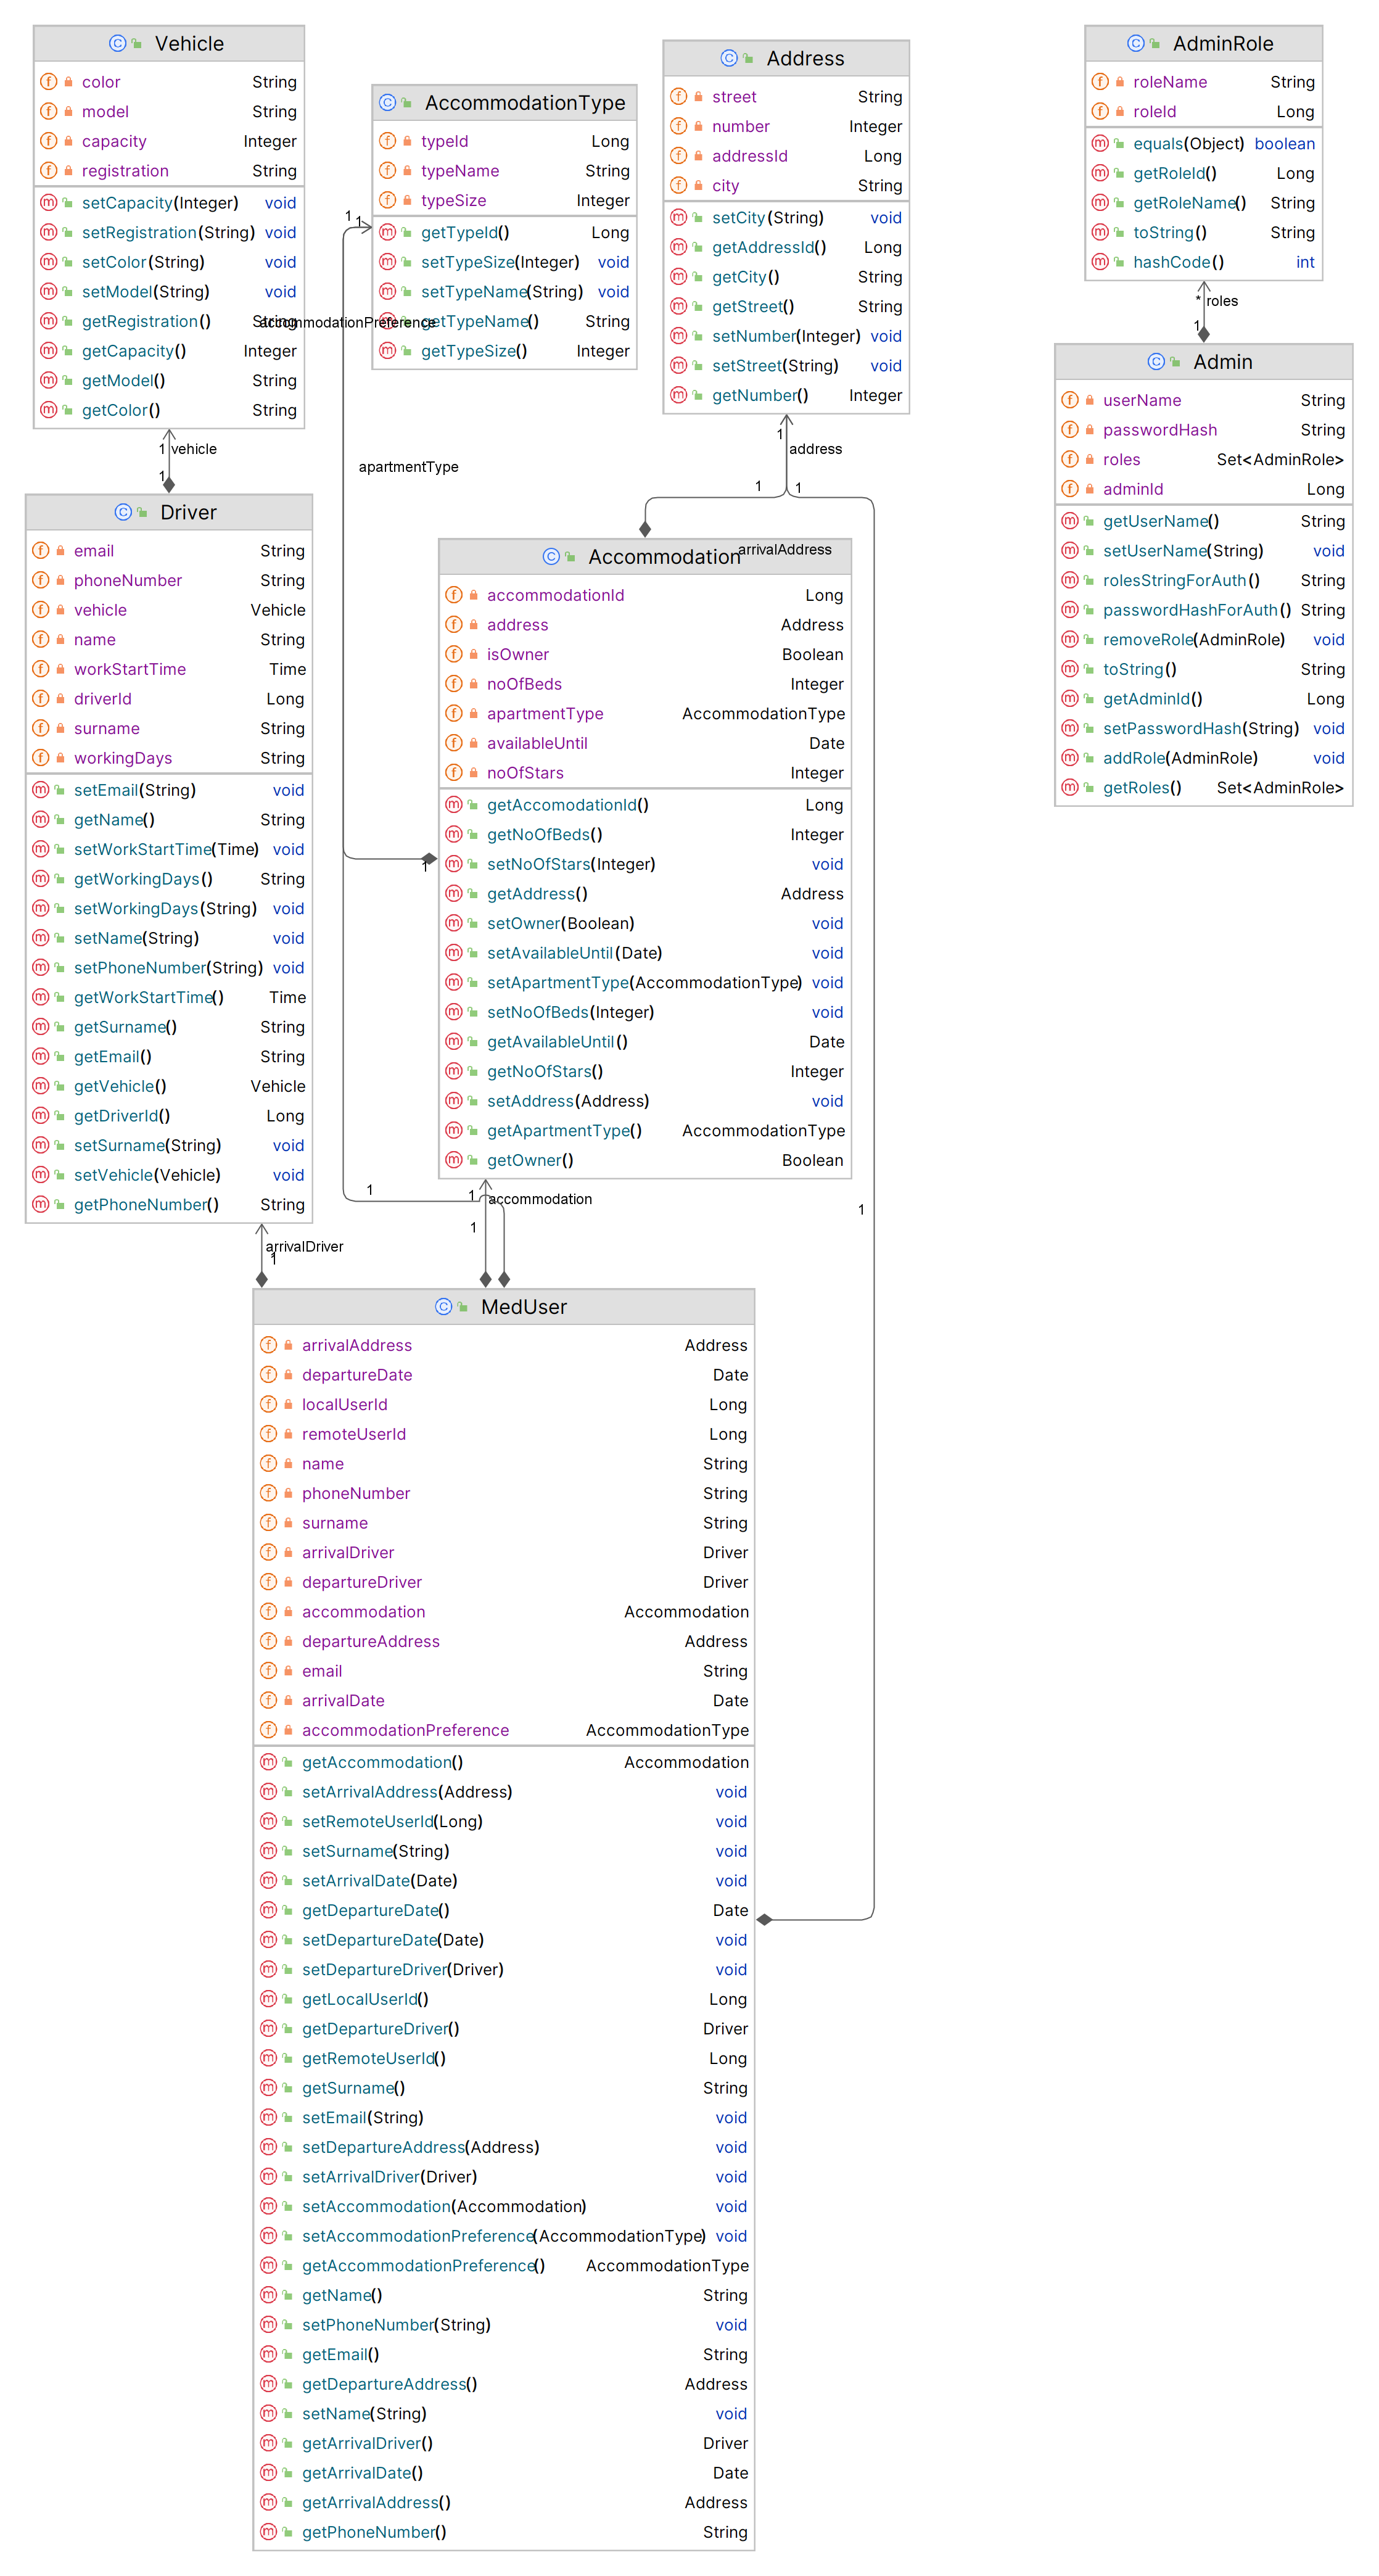
\includegraphics[width=\textwidth]{slike/domain.PNG}
				\caption{Dijagram razreda - Models}
				\label{domainDiagram}
			\end{figure}
			
			{Modeli predstavljaju strukturu baze podataka u našoj aplikaciji. Tako imamo klase: \textit{Admin, MedUser, Accomomodation te Transport} sa svojim privatnim atributima te javnim metodama. Tako na primjer \textit{Admin} ima svoj ID, nadimak, ime te pripadajuće uloge, koje mogu biti smještajni administrator(ima najveće ovlasti), korisnički administrator te prijevozni administrator, što je sadržano u enumeraciji \textit{AdminRole}. \textit{Accommodation} i \textit{Transport} sadrže sve podatke vezane uz smještaj, odnosno prijevoz, a \textit{MedUser} sadrži sve potrebno za definiranje korisnika medicinskih usluga. }\\
			
			
			
			\textbf{\textit{dio 2. revizije}}\\			
			
			\textit{Prilikom druge predaje projekta dijagram razreda i opisi moraju odgovarati stvarnom stanju implementacije}
			
			
			
			\eject
		
		\section{Dijagram stanja}
			
			
			\textbf{\textit{dio 2. revizije}}\\
			
			\textit{Potrebno je priložiti dijagram stanja i opisati ga. Dovoljan je jedan dijagram stanja koji prikazuje \textbf{značajan dio funkcionalnosti} sustava. Na primjer, stanja korisničkog sučelja i tijek korištenja neke ključne funkcionalnosti jesu značajan dio sustava, a registracija i prijava nisu. }
			
			
			\eject 
		
		\section{Dijagram aktivnosti}
			
			\textbf{\textit{dio 2. revizije}}\\
			
			 \textit{Potrebno je priložiti dijagram aktivnosti s pripadajućim opisom. Dijagram aktivnosti treba prikazivati značajan dio sustava.}
			
			\eject
		\section{Dijagram komponenti}
		
			\textbf{\textit{dio 2. revizije}}\\
		
			 \textit{Potrebno je priložiti dijagram komponenti s pripadajućim opisom. Dijagram komponenti treba prikazivati strukturu cijele aplikacije.}